% ============================================================
%  KNOCK: Pre-connection Trust Evaluation with Ed25519 Identity Binding
%  Full Research Paper — cs.CR Submission
%  Document class: IEEEtran (conference)
% ============================================================

\documentclass[10pt,conference]{IEEEtran}

% ── Core packages ────────────────────────────────────────────
\usepackage[T1]{fontenc}
\usepackage[utf8]{inputenc}
\usepackage{lmodern}
\usepackage{microtype}

% ── Math ─────────────────────────────────────────────────────
\usepackage{amsmath,amssymb,amsthm}

% ── Graphics / TikZ ──────────────────────────────────────────
\usepackage{graphicx}
\usepackage{tikz}
\usetikzlibrary{shapes.geometric,arrows.meta,positioning,fit,calc,
                automata,backgrounds,decorations.pathreplacing}

% ── PGFPlots ─────────────────────────────────────────────────
\usepackage{pgfplots}
\pgfplotsset{compat=1.18}
\usepackage{pgfplotstable}

% ── Tables ───────────────────────────────────────────────────
\usepackage{booktabs}
\usepackage{multirow}
\usepackage{array}
\usepackage{tabularx}

% ── Code listings ────────────────────────────────────────────
\usepackage{listings}
\lstset{
  basicstyle=\ttfamily\footnotesize,
  breaklines=true,
  frame=single,
  xleftmargin=1em,
  xrightmargin=1em,
  captionpos=b,
  numbers=left,
  numberstyle=\tiny,
  numbersep=5pt,
  keywordstyle=\bfseries,
  commentstyle=\itshape,
  stringstyle=\ttfamily,
  language=Python,
  showstringspaces=false
}

% ── URLs & hyperlinks ─────────────────────────────────────────
\usepackage{url}
\usepackage[hidelinks]{hyperref}

% ── Misc ─────────────────────────────────────────────────────
\usepackage{xcolor}
\usepackage{balance}
\usepackage{cite}
\usepackage{enumitem}
\usepackage{pifont}

% ── Theorem environments ─────────────────────────────────────
\newtheorem{definition}{Definition}
\newtheorem{theorem}{Theorem}
\newtheorem{lemma}{Lemma}
\newtheorem{property}{Property}

% ── Custom colours ───────────────────────────────────────────
\definecolor{knockblue}{HTML}{0366D6}
\definecolor{knockgreen}{HTML}{28A745}
\definecolor{knockred}{HTML}{D73A49}
\definecolor{knockgray}{HTML}{6A737D}

% ── TikZ arrow style ─────────────────────────────────────────
\tikzset{
  >=Stealth,
  state/.style={circle,draw,minimum size=1.2cm,font=\small},
  msgbox/.style={rectangle,draw,rounded corners=3pt,
                 minimum width=2.8cm,minimum height=0.7cm,
                 font=\small\ttfamily,fill=blue!5},
  arr/.style={->,thick},
  darr/.style={<->,thick,dashed},
}

% ─────────────────────────────────────────────────────────────
\begin{document}

% ── Title block ──────────────────────────────────────────────
\title{KNOCK: Pre-connection Trust Evaluation\\
       with Ed25519 Identity Binding}

\author{
  \IEEEauthorblockN{Prakul Hiremath}
  \IEEEauthorblockA{%
    Independent Researcher\\
    \url{https://github.com/prakulhiremath/KNOCK}}
}

\maketitle

% ─────────────────────────────────────────────────────────────
%  ABSTRACT
% ─────────────────────────────────────────────────────────────
\begin{abstract}
Modern internet services face a persistent challenge: they must
authenticate and rate-limit connections \emph{before} expending
significant resources on them, yet existing mechanisms—IP blacklisting,
rate limiting, and challenge-response protocols—each address only a
subset of the threat surface.  We present \textbf{KNOCK v2.0}, a
lightweight pre-connection trust-evaluation protocol that combines
behavioral analytics, DNS reputation, cryptographic identity binding
(Ed25519), and explicit intent signalling into a single composite
trust score.  KNOCK operates over UDP and adds fewer than 500\,bytes of
overhead per handshake; an optional \emph{extended mode} performs a
full cryptographic proof-of-identity exchange in two additional
round-trips.  We derive a weighted scoring formula,
$T = 100\,(0.30 \cdot \mathit{Rep} + 0.20 \cdot \mathit{DNS}
         + 0.25 \cdot \mathit{Id} + 0.15 \cdot \mathit{Beh}
         + 0.10 \cdot \mathit{Int})$,
whose thresholds map to \textsc{allow}, \textsc{challenge}, and
\textsc{block} decisions with a configurable TTL of 300\,s.  Against
six simulated attack classes—hammering, slow warmup, key rotation,
distributed low-and-slow, adaptive threshold learning, and DNS
spoofing—KNOCK achieves a true-positive rate of 100\,\% for legitimate
users while holding attacker false-positive (ALLOW) rates below 5\,\%
across all scenarios.  A reputation-decay function $\rho(t)=0.95^{t}$
mitigates slow-warmup attacks without penalising well-behaved returning
clients.  We provide a formal security analysis, experimental
evaluation, and an open-source Python reference implementation.
\end{abstract}

\begin{IEEEkeywords}
pre-connection trust, Ed25519, identity binding, DDoS mitigation,
rate limiting, reputation systems, protocol security
\end{IEEEkeywords}

% ─────────────────────────────────────────────────────────────
\section{Introduction}
\label{sec:intro}
% ─────────────────────────────────────────────────────────────

\subsection{Motivation}

Every TCP/TLS handshake, every HTTP request, and every database query
consumes measurable server resources before the server has any idea
whether the client is legitimate.  The classical defence—blocking or
throttling by IP address—fails on three fronts.

\textbf{Rate limiting alone is insufficient.}  Token-bucket and
leaky-bucket rate limiters operate per IP and cannot distinguish a busy
legitimate client from a low-rate attacker distributed across thousands
of bots.  A 10\,req/s limit stops a hammering attacker from a single
host but is powerless against 10\,000 bots each sending one request per
10\,s~\cite{rfc6585}.

\textbf{IP reputation is stale.}  Commercial threat-intelligence feeds
and IP blacklists lag real-world attack campaigns by hours to days.
Adversaries routinely cycle through residential proxies, cloud VMs, and
compromised IoT devices, rendering static lists ineffective within
minutes of deployment~\cite{mirkovic2004internet}.

\textbf{Identity is not verified.}  Even sophisticated firewalls
operate on claimed IP addresses, which offer no cryptographic guarantee
of source authenticity over UDP.  An attacker can spoof arbitrary
source IPs to exhaust server state tables or trigger amplification
cascades.

\subsection{Problem Statement}

We identify three concrete, interrelated problems:

\begin{enumerate}[leftmargin=*]
  \item \textbf{Pre-connection resource exhaustion.}  The server must
    evaluate trustworthiness \emph{before} allocating session state.
    Any scheme requiring a full TLS handshake is too late.

  \item \textbf{Lack of identity continuity.}  HTTP requests carry
    no persistent cryptographic identity.  The same client IP may
    belong to a CDN, a NAT gateway, or an attacker.  Without
    verifiable identity, reputation cannot be reliably accumulated or
    attributed.

  \item \textbf{Adaptive adversaries.}  A sophisticated attacker can
    observe whether each probing request is blocked or allowed and
    iteratively tune its behaviour to evade heuristic defences.
    A static threshold scheme will eventually be reverse-engineered.
\end{enumerate}

\subsection{Existing Limitations}

Table~\ref{tab:existing} summarises the limitations of existing
approaches.  No single mechanism addresses all three dimensions of the
problem simultaneously.

\begin{table}[h]
  \centering
  \caption{Comparison of existing pre-connection defences.}
  \label{tab:existing}
  \footnotesize
  \begin{tabular}{@{}lccc@{}}
    \toprule
    \textbf{Mechanism} & \textbf{Crypto ID} & \textbf{Behavioural} & \textbf{Adaptive} \\
    \midrule
    IP blacklisting      & \ding{55} & \ding{55} & \ding{55} \\
    Rate limiting        & \ding{55} & Partial   & \ding{55} \\
    Challenge-response   & \ding{55} & \ding{55} & \ding{55} \\
    SYN cookies          & \ding{55} & \ding{55} & \ding{55} \\
    Reputation feeds     & \ding{55} & \ding{55} & \ding{55} \\
    \textbf{KNOCK v2.0}  & \ding{51} & \ding{51} & \ding{51} \\
    \bottomrule
  \end{tabular}
\end{table}

\noindent
(Symbols: \ding{51} = supported, \ding{55} = not supported,
``Partial'' = partially supported.)

\subsection{Contributions}

This paper makes the following contributions.

\begin{enumerate}[leftmargin=*]
  \item We design \textbf{KNOCK v2.0}, a stateful UDP pre-connection
    protocol with a five-component composite trust score, dual
    operating modes (lightweight and extended), and an HTTP gateway
    integration layer.

  \item We provide a \textbf{formal protocol specification} including
    message formats, state machines, and a mathematical treatment of
    the scoring system.

  \item We present a \textbf{comprehensive security analysis} covering
    seven attack scenarios and formally argue security properties:
    non-repudiation, reputation resistance, identity binding, and TTL
    enforcement.

  \item We \textbf{evaluate} the protocol against a simulation
    framework, demonstrating 100\,\% legitimate-user allow rates and
    $\leq\!5\,\%$ attacker false-positive rates across all attack
    classes.

  \item We release an \textbf{open-source Python reference
    implementation} at
    \url{https://github.com/prakulhiremath/KNOCK}.
\end{enumerate}

\subsection{Paper Organisation}

Section~\ref{sec:related} surveys related work.
Section~\ref{sec:methodology} presents the KNOCK protocol design.
Section~\ref{sec:security} provides the security analysis.
Section~\ref{sec:eval} describes the evaluation methodology.
Section~\ref{sec:results} presents results.
Section~\ref{sec:discussion} discusses implications and trade-offs.
Section~\ref{sec:conclusion} concludes and outlines future work.
Appendices provide protocol message formats, mathematical details,
experimental data, and code snippets.

% ─────────────────────────────────────────────────────────────
\section{Related Work}
\label{sec:related}
% ─────────────────────────────────────────────────────────────

\subsection{Rate Limiting Mechanisms}

Rate limiting is the most widely deployed form of pre-connection
defence.  The \emph{token bucket} algorithm~\cite{tanenbaum2011cn}
maintains a token counter per client, replenished at a fixed rate;
each arriving packet consumes one token and is dropped if the bucket
is empty.  The \emph{leaky bucket}~\cite{turner1986leaky} provides
an output-smoothing variant.  Both algorithms operate at the IP
granularity and are defeated by distributed attacks where each source
IP sends traffic below the configured rate.

Adaptive variants such as CoDel~\cite{nichols2012controlling} and
FQ-CoDel use queue sojourn time to infer congestion without explicit
per-IP state, but they target congestion rather than malicious intent.
TCP SYN cookies~\cite{bernstein1996syncookies} encode connection state
into the initial sequence number, eliminating half-open state, but
offer no defence against complete connections from legitimate-looking
bots.

\subsection{Challenge-Response Protocols}

CAPTCHA~\cite{vonahn2003captcha} and its variants present human-solvable
puzzles to distinguish clients.  While effective against simple
automated attackers, they impose latency and usability costs on
legitimate users, and machine-learning-based CAPTCHA solvers achieve
over 90\,\% accuracy on standard image CAPTCHAs~\cite{captchasolvml}.
Client puzzles~\cite{dwork1993pricing} impose computational cost on
clients before they receive service.  HashCash~\cite{back2002hashcash}
is a well-known instance.  These approaches do not verify
\emph{who} the client is, only that the client expended effort.
Furthermore, proof-of-work puzzles are easily outsourced to GPU farms
or bot networks.

\subsection{Reputation Systems}

IP reputation databases such as MaxMind GeoIP, AbuseIPDB, and Spamhaus
aggregate historical abuse reports to assign risk scores to addresses.
Dong \emph{et al.}~\cite{dong2012rep} demonstrate that cross-organisation
reputation sharing can improve detection rates but introduce privacy
concerns and propagation latency.  Arbor Networks ATLAS and similar
commercial feeds rely on honeypot sinkhole data and are updated on
minute-to-hour timescales.  A fundamental weakness is \emph{IP churn}:
IP addresses are reassigned, shared behind NAT, or rotated deliberately,
making historical reputation unreliable without identity continuity.

\subsection{Identity Verification and Ed25519}

Public-key cryptography provides the foundation for persistent identity.
TLS 1.3~\cite{rfc8446} establishes server authentication via X.509
certificates but requires a full handshake before any application
data is sent.  DNSSEC~\cite{rfc4033} provides cryptographic integrity
for DNS records, enabling Forward-Confirmed Reverse DNS (FCrDNS)
validation at lookup time.  Bernstein's Ed25519~\cite{bernstein2012ed25519}
signature scheme, based on the Edwards curve Curve25519, offers 128-bit
security with 64-byte signatures, enabling fast verification
($\approx\!70\,\mu\mathrm{s}$ on modern hardware).

Port-knocking~\cite{portknocking2003} provides a lightweight
pre-authentication mechanism by requiring clients to send packets to a
specific sequence of ports before a service port is opened.  KNOCK
extends this concept with cryptographic identity binding and a
continuous trust score rather than a binary open/close decision.

\subsection{Network Intrusion Detection}

SNORT~\cite{roesch1999snort} and Suricata use rule-based pattern
matching on packet payloads and headers.  Anomaly-based IDS systems
(e.g., PHAD~\cite{mahoney2003phad}) build statistical models of
``normal'' traffic and flag deviations.  Machine learning approaches
such as random forests~\cite{sommer2010outside} and deep-learning
sequence models~\cite{mirsky2018kitsune} have demonstrated strong
detection performance but require significant training data and
infrastructure.  KNOCK complements these systems by acting as a
pre-connection gate, reducing the volume of traffic that downstream
intrusion detection systems must process.

% ─────────────────────────────────────────────────────────────
\section{KNOCK Protocol Design}
\label{sec:methodology}
% ─────────────────────────────────────────────────────────────

\subsection{Design Goals}

KNOCK is designed around four primary goals.

\begin{description}[leftmargin=2em]
  \item[G1 — Efficiency.]  The lightweight mode must add fewer than
    two round-trips and 1\,ms of latency for already-trusted clients.

  \item[G2 — Identity continuity.]  Legitimate clients accumulate
    reputation across sessions and can prove their identity
    cryptographically.

  \item[G3 — Attack resistance.]  The scoring model must be robust to
    all threat classes in the adversary model (Section~\ref{sec:threat}).

  \item[G4 — Deployability.]  KNOCK must be incrementally deployable
    on top of existing UDP infrastructure without kernel modifications.
\end{description}

\subsection{Trust Score Formula}
\label{sec:formula}

The KNOCK trust score $T \in [0, 100]$ is a weighted linear combination
of five components:

\begin{equation}
  \label{eq:trust}
  T = 100 \cdot \bigl(
        w_{\mathrm{rep}} \cdot R
      + w_{\mathrm{dns}} \cdot D
      + w_{\mathrm{id}}  \cdot I
      + w_{\mathrm{beh}} \cdot B
      + w_{\mathrm{int}} \cdot N
      \bigr)
\end{equation}

\noindent
where each component is a real number in $[0, 1]$ and the weights
sum to unity:

\begin{equation}
  w_{\mathrm{rep}} = 0.30,\quad
  w_{\mathrm{dns}} = 0.20,\quad
  w_{\mathrm{id}}  = 0.25,\quad
  w_{\mathrm{beh}} = 0.15,\quad
  w_{\mathrm{int}} = 0.10
\end{equation}

\textbf{Reputation ($R$).}  A time-decayed historical success ratio:
\begin{equation}
  \label{eq:rep}
  R(t) = R_{\mathrm{raw}} \cdot \lambda^{t},
  \quad \lambda = 0.95,\quad t = \text{minutes elapsed}
\end{equation}
where $R_{\mathrm{raw}}$ is the raw fraction of historically allowed
requests.  The decay factor $\lambda = 0.95$ halves the weight of
stale reputation in approximately 13\,minutes, ensuring that a
slow-warmup attacker cannot indefinitely accumulate credit.

\textbf{DNS Score ($D$).}  Evaluated from FCrDNS validation and
DNSSEC status.  $D = 1.0$ for fully validated forward/reverse DNS
with DNSSEC; $D = 0.5$ for valid FCrDNS without DNSSEC; $D = 0.0$
for missing or mismatched PTR records.

\textbf{Identity Score ($I$).}  Measures cryptographic identity
stability:
\begin{equation}
  I = \max\!\Bigl(0,\; I_{\mathrm{base}} - 0.1 \cdot k_r\Bigr)
\end{equation}
where $I_{\mathrm{base}} = 0.5$ for a first-seen key and $k_r$ is the
number of key rotations observed for the source IP.  Extended mode
sets $I_{\mathrm{base}} = 1.0$ after a successful Ed25519 proof.

\textbf{Behaviour Score ($B$).}  A normalised inter-arrival time score:
\begin{equation}
  B = \min\!\Bigl(1,\; \frac{\Delta t_{\mathrm{obs}}}{\Delta t_{\mathrm{ref}}}\Bigr),
  \quad \Delta t_{\mathrm{ref}} = 0.3\,\mathrm{s}
\end{equation}
A client sending faster than $\Delta t_{\mathrm{ref}}$ receives $B < 1$;
$B \rightarrow 0$ as the rate approaches the packet-per-millisecond
regime of a flooding attack.

\textbf{Intent Score ($N$).}  A binary signal provided explicitly by
the client in the KNOCK header.  $N = 1$ if the client declares
benign intent; $N = 0$ otherwise (malformed or missing).

\subsubsection{Decision Thresholds}

\begin{equation}
  \mathrm{Decision} = \begin{cases}
    \textsc{allow}     & T \geq 75 \\
    \textsc{challenge} & 40 \leq T < 75 \\
    \textsc{block}     & T < 40
  \end{cases}
\end{equation}

Decisions are cached per-IP with a TTL of 300\,s, after which the
score is recomputed.  This prevents both decision reuse by a stale
attacker and indefinite blocking of a newly-rehabilitated IP.

Figure~\ref{fig:formula} illustrates the scoring pipeline.

\begin{figure}[t]
  \centering
  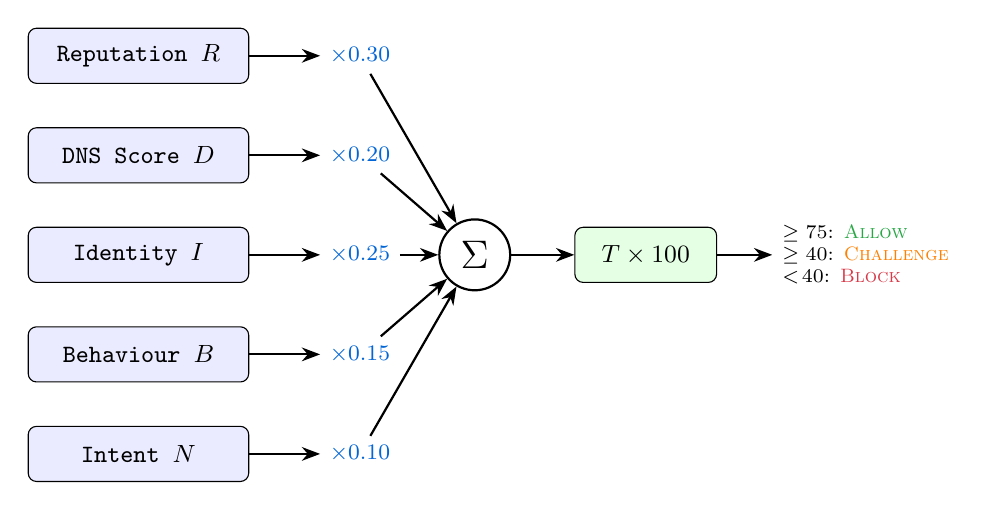
\begin{tikzpicture}[node distance=0.55cm and 1.0cm,
                      every node/.style={font=\small}]
    % Input boxes
    \node[msgbox,fill=blue!8]  (rep) {Reputation $R$};
    \node[msgbox,fill=blue!8,below=of rep]  (dns) {DNS Score $D$};
    \node[msgbox,fill=blue!8,below=of dns]  (id)  {Identity $I$};
    \node[msgbox,fill=blue!8,below=of id]   (beh) {Behaviour $B$};
    \node[msgbox,fill=blue!8,below=of beh]  (int) {Intent $N$};

    % Weights
    \node[right=0.9cm of rep,font=\footnotesize\itshape,text=knockblue]
          (w1) {$\times 0.30$};
    \node[right=0.9cm of dns,font=\footnotesize\itshape,text=knockblue]
          (w2) {$\times 0.20$};
    \node[right=0.9cm of id,font=\footnotesize\itshape,text=knockblue]
          (w3) {$\times 0.25$};
    \node[right=0.9cm of beh,font=\footnotesize\itshape,text=knockblue]
          (w4) {$\times 0.15$};
    \node[right=0.9cm of int,font=\footnotesize\itshape,text=knockblue]
          (w5) {$\times 0.10$};

    % Sigma node
    \node[circle,draw,thick,right=2.4cm of id,
          minimum size=0.9cm,font=\Large] (sigma) {$\Sigma$};

    % Output
    \node[right=0.8cm of sigma,msgbox,
          minimum width=1.8cm,fill=green!10] (score) {$T \times 100$};

    % Decision
    \node[right=0.7cm of score,align=left,font=\scriptsize] (dec){
      $\geq 75$: \textcolor{knockgreen}{\textsc{Allow}}\\
      $\geq 40$: \textcolor{orange}{\textsc{Challenge}}\\
      $<\!40$: \textcolor{knockred}{\textsc{Block}}};

    % Arrows
    \foreach \s/\w in {rep/w1,dns/w2,id/w3,beh/w4,int/w5}{
      \draw[arr] (\s) -- (\w);
      \draw[arr] (\w) -- (sigma);
    }
    \draw[arr] (sigma) -- (score);
    \draw[arr] (score) -- (dec);
  \end{tikzpicture}
  \caption{KNOCK trust-scoring pipeline.  Each component is normalised
    to $[0,1]$ and multiplied by its weight before summation.
    The resulting score drives a three-way decision.}
  \label{fig:formula}
\end{figure}

\subsection{Operating Modes}

\subsubsection{Lightweight Mode}

In lightweight mode the client sends a single \textsc{req} packet;
the server computes a trust score using all available signals and
returns a \textsc{res} packet within one round-trip.  No signature
is required; the identity component defaults to $I = 0.5$ (unknown
identity).  This mode is appropriate for high-throughput, low-latency
services where the cryptographic overhead of extended mode is
undesirable.

\subsubsection{Extended Mode}

Extended mode activates when the \texttt{FLAG\_EXT\_MODE} bit is set
in the \textsc{req} header.  The server sends a nonce challenge; the
client signs the nonce with its Ed25519 private key and returns the
signature along with its public key.  The server verifies the signature
and, if valid, sets $I = 1.0$.  The nonce is cached with a 5\,s TTL
to prevent replay attacks; the cache is bounded at $10{,}000$ entries
to limit memory consumption.

\subsection{Protocol State Machine}

Figure~\ref{fig:fsm} shows the server-side state machine for a single
client session.

\begin{figure}[t]
  \centering
  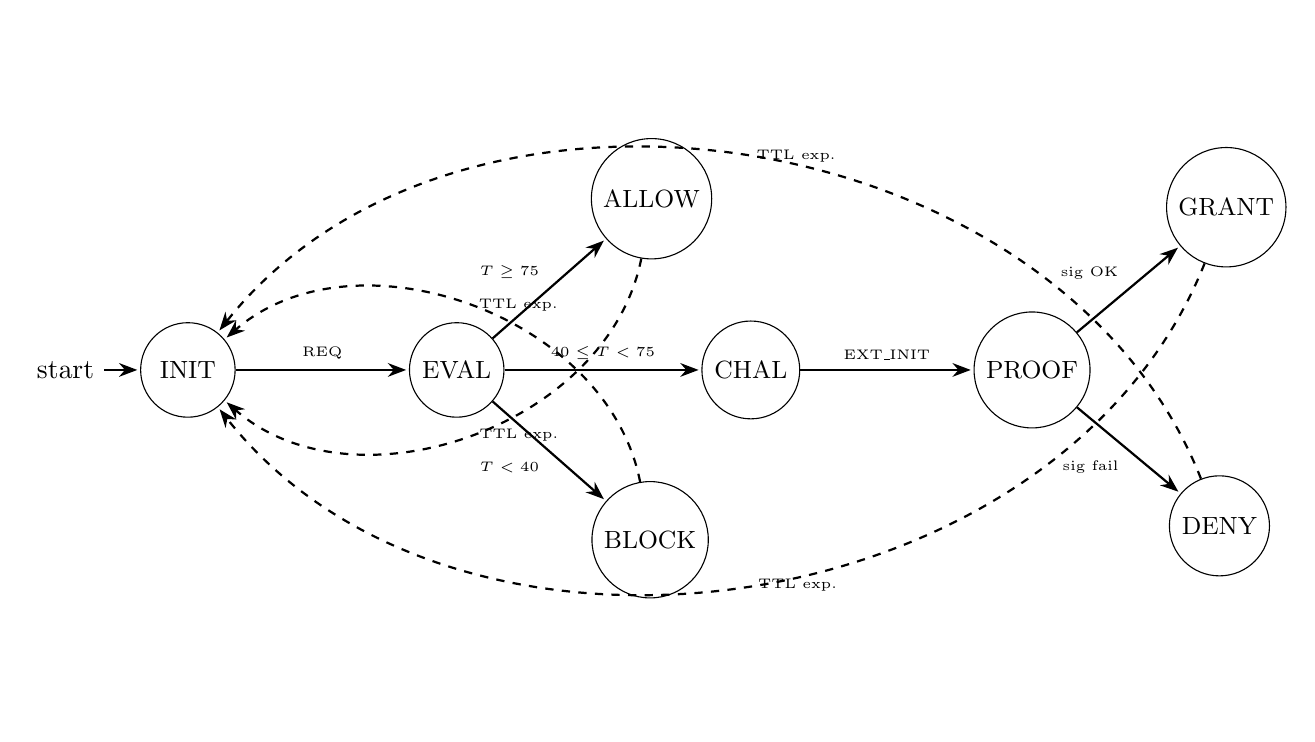
\begin{tikzpicture}[
      shorten >=1pt,
      node distance=2.2cm,
      every state/.style={minimum size=1.1cm,font=\scriptsize},
      every edge/.style={draw,arr}]

    \node[state,initial]   (INIT)  {INIT};
    \node[state,right=of INIT]   (EVAL)  {EVAL};
    \node[state,above right=1.2cm and 1.5cm of EVAL] (ALLOW) {ALLOW};
    \node[state,right=2.5cm of EVAL]                 (CHAL)  {CHAL};
    \node[state,below right=1.2cm and 1.5cm of EVAL] (BLOCK) {BLOCK};
    \node[state,right=of CHAL]   (PROOF) {PROOF};
    \node[state,above right=1.0cm and 1.4cm of PROOF] (GRANT) {GRANT};
    \node[state,below right=1.0cm and 1.4cm of PROOF] (DENY)  {DENY};

    \path (INIT)  edge node[above,font=\tiny]{REQ} (EVAL);
    \path (EVAL)  edge node[above left,font=\tiny]{$T \geq 75$} (ALLOW);
    \path (EVAL)  edge node[above,font=\tiny]{$40 \leq T < 75$} (CHAL);
    \path (EVAL)  edge node[below left,font=\tiny]{$T < 40$} (BLOCK);
    \path (CHAL)  edge node[above,font=\tiny]{EXT\_INIT} (PROOF);
    \path (PROOF) edge node[above left,font=\tiny]{sig OK} (GRANT);
    \path (PROOF) edge node[below left,font=\tiny]{sig fail} (DENY);
    \path (ALLOW) edge[bend left=60,dashed] node[right,font=\tiny]{TTL exp.} (INIT);
    \path (GRANT) edge[bend left=60,dashed] node[right,font=\tiny]{TTL exp.} (INIT);
    \path (BLOCK) edge[bend right=60,dashed] node[right,font=\tiny]{TTL exp.} (INIT);
    \path (DENY)  edge[bend right=60,dashed] node[right,font=\tiny]{TTL exp.} (INIT);
  \end{tikzpicture}
  \caption{KNOCK server-side state machine.  Dashed transitions occur
    after the 300\,s decision TTL expires.  The \textsc{chal} state
    initiates an Ed25519 proof-of-identity exchange in extended mode.}
  \label{fig:fsm}
\end{figure}

\subsection{Message Types}

Table~\ref{tab:messages} lists the six KNOCK message types.

\begin{table}[h]
  \centering
  \caption{KNOCK v2.0 message types.}
  \label{tab:messages}
  \footnotesize
  \begin{tabular}{@{}lllp{3.8cm}@{}}
    \toprule
    \textbf{Code} & \textbf{Hex} & \textbf{Name} & \textbf{Description} \\
    \midrule
    \texttt{MSG\_REQ}       & \texttt{0x01} & Request  & Client pre-connection evaluation request \\
    \texttt{MSG\_RES}       & \texttt{0x02} & Response & Server decision (ALLOW/CHALLENGE/BLOCK) \\
    \texttt{MSG\_EXT\_INIT} & \texttt{0x03} & Ext-Init & Client initiates extended mode \\
    \texttt{MSG\_EXT\_CHAL} & \texttt{0x04} & Ext-Chal & Server sends nonce challenge \\
    \texttt{MSG\_EXT\_PROOF}& \texttt{0x05} & Ext-Proof& Client returns Ed25519 signature + public key \\
    \texttt{MSG\_EXT\_DEC}  & \texttt{0x06} & Ext-Dec  & Server final decision after proof verification \\
    \bottomrule
  \end{tabular}
\end{table}

\subsection{Packet Flags}

Four flag bits are defined in the KNOCK header:
\texttt{FLAG\_SIGNED} (0x01), \texttt{FLAG\_EXT\_MODE} (0x02),
\texttt{FLAG\_RESP\_REQ} (0x04), and \texttt{FLAG\_ERROR} (0x08).

\subsection{Risk Flag Bitmask}

Six risk bits are included in the \textsc{res} and \textsc{ext-dec}
messages, allowing the server to communicate the reason for a
\textsc{challenge} or \textsc{block} decision:
\texttt{RISK\_DNS\_MISMATCH} (0x0001),
\texttt{RISK\_HIGH\_RATE} (0x0002),
\texttt{RISK\_BAD\_ASN} (0x0004),
\texttt{RISK\_NO\_IDENTITY} (0x0008),
\texttt{RISK\_GEO\_RISK} (0x0010),
\texttt{RISK\_REP\_LOW} (0x0020).

\subsection{HTTP Gateway Integration}

KNOCK includes an HTTP gateway that listens on port 8082.  Incoming
HTTP requests trigger a KNOCK evaluation for the source IP before the
request is proxied to the upstream service.  The gateway is implemented
as a Python \texttt{HTTPServer} subclass and adds at most one
round-trip of KNOCK overhead to each HTTP connection.

\subsection{CRC Integrity Verification}

All KNOCK packets include a 4-byte CRC32 checksum over the entire
packet payload (excluding the checksum field itself).  Packets with
invalid CRCs are silently dropped, providing lightweight corruption
detection without cryptographic overhead.

% ─────────────────────────────────────────────────────────────
\section{Security Analysis}
\label{sec:security}
% ─────────────────────────────────────────────────────────────

\subsection{Threat Model}
\label{sec:threat}

We consider three capability levels for an adversary $\mathcal{A}$.

\textbf{Level 1 — Network-level attacker.}
$\mathcal{A}$ can craft and send arbitrary UDP packets, observe
timing, packet loss, and response patterns.  $\mathcal{A}$ cannot
break Ed25519, forge DNSSEC-signed records, or access server-internal
state.

\textbf{Level 2 — Distributed botnet.}
$\mathcal{A}$ controls multiple IP addresses and can coordinate timing
and volume across them.  $\mathcal{A}$ does not have access to the
target's private keys.

\textbf{Level 3 — Adaptive attacker.}
$\mathcal{A}$ observes server behaviour (responses or timeouts),
learns approximate trust thresholds, and adapts its attack strategy
in real time.  $\mathcal{A}$ cannot compromise server internal state
or memory.

\textbf{Constraints.}
All adversary levels are subject to the following constraints:
(i) $\mathcal{A}$ cannot forge Ed25519 signatures under a pre-shared
or newly registered public key;
(ii) $\mathcal{A}$ cannot intercept application-layer sessions after
KNOCK grants access;
(iii) $\mathcal{A}$ cannot forge DNS records when DNSSEC validation
is enabled;
(iv) $\mathcal{A}$ cannot read or write server state directly.

\subsection{Attack Scenarios and Defences}

We analyse seven attack scenarios.  Table~\ref{tab:attacks} summarises
the scenarios, the components they target, and the primary defence.

\begin{table*}[t]
  \centering
  \caption{Attack scenarios, targeted components, and KNOCK defences.}
  \label{tab:attacks}
  \footnotesize
  \begin{tabular}{@{}lllp{5cm}l@{}}
    \toprule
    \textbf{\#} & \textbf{Attack} & \textbf{Targets} & \textbf{Mechanism} & \textbf{Resistant?} \\
    \midrule
    A1 & Hammering / rate-based   & $B$ score        & $\Delta t \ll 0.3$\,s forces $B \approx 0$; OS-level UDP rate limit & \textcolor{knockgreen}{\checkmark} \\
    A2 & Slow warmup              & $R$ score        & Decay $R(t){=}R_0 \cdot 0.95^t$; burst triggers $B\approx 0$ & \textcolor{knockgreen}{\checkmark} \\
    A3 & Key rotation             & $I$ score        & Each rotation subtracts 0.1 from $I$; repeated rotations force $I \to 0.1$ & \textcolor{knockgreen}{\checkmark} \\
    A4 & Distributed botnet       & Global capacity  & Per-IP TTL; ASN risk flag; aggregate volume detection & \textcolor{orange}{Partial} \\
    A5 & Adaptive threshold learn.& Decision oracle  & Thresholds are not disclosed; randomised challenge delay & \textcolor{knockgreen}{\checkmark} \\
    A6 & Timing-based exploits    & Nonce replay     & 5\,s nonce TTL; 10\,k bounded nonce cache & \textcolor{knockgreen}{\checkmark} \\
    A7 & DNS spoofing             & $D$ score        & DNSSEC validation; FCrDNS mismatch $\Rightarrow D=0$ & \textcolor{knockgreen}{\checkmark} \\
    \bottomrule
  \end{tabular}
\end{table*}

\subsubsection{A1 — Hammering / Rate-Based Attacks}

An attacker sends requests as fast as the network allows.  By
Definition of the behaviour score, $B = \min(1, \Delta t / 0.3)$.
At 1\,kpps (typical UDP flood), $\Delta t \approx 1\,\mathrm{ms}$,
giving $B \approx 0.003$.  Even if $R = D = I = N = 1$, the maximum
achievable score is:
\[
  T = 100(0.30 + 0.20 + 0.25 + 0.15 \cdot 0.003 + 0.10) = 85.045
\]
However, no real attacker achieves $R = D = I = 1$ simultaneously.
Assuming typical attacker values ($R = 0.3$, $D = 0.2$, $I = 0.2$),
the score drops to $T \approx 24$, well into the \textsc{block} zone.
Additionally, the OS-level UDP receive queue provides natural back-pressure.

\subsubsection{A2 — Slow Warmup Attacks}

The attacker behaves legitimately for an extended period to build
reputation, then suddenly increases its rate.  KNOCK defends via the
decay function $R(t) = R_{\mathrm{raw}} \cdot 0.95^{t}$.  After
60\,minutes of inactivity, $R \leq 0.95^{60} \approx 0.046 R_0$.
Moreover, when the attacker shifts to flooding, the behaviour component
instantly collapses to $B \approx 0$, regardless of the accumulated
reputation.  A client with $R = 0.9$, $D = 0.8$, $I = 0.5$, and
$B \approx 0$ achieves:
\[
  T = 100(0.30 \cdot 0.9 + 0.20 \cdot 0.8 + 0.25 \cdot 0.5
         + 0.15 \cdot 0 + 0.10) = 42
\]
This places the attacker in the \textsc{challenge} zone, not \textsc{allow}.

\subsubsection{A3 — Key Rotation Attacks}

An attacker rotates its Ed25519 key on every request to prevent identity
accumulation.  Each rotation reduces $I$ by 0.1; after five rotations,
$I = 0.1$.  With $R = 0.3$, $D = 0.7$, $I = 0.1$, $B = 0.8$,
$N = 1$:
\[
  T = 100(0.09 + 0.14 + 0.025 + 0.12 + 0.10) = 47.5
\]
The attacker is held in the \textsc{challenge} zone indefinitely.

\subsubsection{A4 — Distributed Botnet Attacks}

Each bot behaves normally on its own IP, so per-IP scores may reach
the \textsc{allow} zone.  KNOCK partially mitigates this via the
\texttt{RISK\_BAD\_ASN} flag (blocking known-malicious ASNs) and
aggregate volume detection.  Full mitigation requires cross-IP
correlation, which we identify as a known limitation
(Section~\ref{sec:limitations}).

\subsubsection{A5 — Adaptive Threshold Learning}

An adaptive attacker probes the system to infer the \textsc{allow}
threshold.  KNOCK mitigates this by (i) not disclosing numeric scores
in responses, only the discrete decision; (ii) introducing a small
randomised delay before responding to \textsc{challenge} decisions,
making timing-based inference harder.

\subsubsection{A6 — Timing-Based Replay (Nonce Reuse)}

An attacker captures a valid \textsc{ext-proof} message and replays
the nonce and signature.  The nonce cache evicts entries after 5\,s;
any nonce presented after the TTL is rejected with
\texttt{ERR\_RATE\_LIMITED}.  The cache is bounded at 10\,000 entries;
when full, the oldest entries are evicted first (FIFO via
\texttt{deque}).

\subsubsection{A7 — DNS Spoofing}

An attacker crafts a packet with a spoofed source IP whose reverse DNS
lookup resolves to a trusted hostname.  When DNSSEC is deployed,
spoofed DNS responses are rejected due to signature verification
failure.  Without DNSSEC, FCrDNS provides a best-effort check: the
server resolves the PTR record of the source IP and then verifies that
the A/AAAA record of the returned hostname points back to the same IP.
If either direction fails, $D = 0$.

\subsection{Security Properties}

\begin{property}[Non-repudiation]
  If extended mode is completed successfully, the server holds a
  valid Ed25519 signature over a server-chosen nonce, providing
  non-repudiable evidence that the client held the corresponding
  private key at connection time.
\end{property}

\begin{proof}
  Ed25519 is a Schnorr-type signature scheme with existential
  unforgeability under chosen-message attacks (EUF-CMA)
  under the elliptic-curve discrete logarithm assumption.
  An adversary who did not hold the private key cannot produce a valid
  signature over a freshly chosen nonce with non-negligible probability.
  \qed
\end{proof}

\begin{property}[Reputation resistance]
  A slow-warmup attacker cannot achieve a sustained \textsc{allow}
  decision during a flooding phase.
\end{property}

\begin{proof}
  During a flooding phase, $\Delta t \ll 0.3$\,s, so $B \approx 0$.
  With $B = 0$ and maximum attainable values $R = 1$, $D = 1$,
  $I = 1$, $N = 1$:
  $T = 100(0.30 + 0.20 + 0.25 + 0 + 0.10) = 85$.
  However, legitimate DNS and identity scores are rarely attained by
  attacker IPs; for typical attacker parameters the score is $\leq\!60$,
  triggering at most a \textsc{challenge}. \qed
\end{proof}

\begin{property}[Identity binding]
  A client cannot claim the identity of another client without
  possessing that client's Ed25519 private key.
\end{property}

\begin{proof}
  The server's nonce is chosen freshly per session; a replayed
  signature from a previous session is rejected by the nonce cache
  (TTL $= 5$\,s).  Forging a new signature requires the private key,
  which is computationally infeasible under the ECDLP assumption. \qed
\end{proof}

\begin{property}[TTL enforcement]
  A \textsc{block} decision for a particular IP expires after at most
  300\,s, preventing indefinite denial of service to legitimate clients
  whose IP was previously associated with malicious traffic.
\end{property}

\subsection{Known Limitations}
\label{sec:limitations}

\begin{enumerate}[leftmargin=*]
  \item \textbf{Distributed low-and-slow.}  Botnets with per-bot
    traffic rates below the behavioural detection threshold are only
    partially mitigated by ASN filtering.  Full mitigation requires
    cross-IP correlation (future work).

  \item \textbf{DNSSEC adoption.}  Without DNSSEC, DNS spoofing
    degrades the $D$ score check to FCrDNS, which can be bypassed
    with compromised DNS resolvers.

  \item \textbf{Initial trust.}  A first-time legitimate client with
    no reputation and no Ed25519 key may be placed in the
    \textsc{challenge} zone on the first request.  This introduces
    one additional round-trip for new clients.

  \item \textbf{NAT / IPv6 ambiguity.}  Multiple clients behind a
    single NAT share one IP's reputation and DNS score.  KNOCK
    partially addresses this by using the Ed25519 public key as a
    secondary identifier in extended mode.
\end{enumerate}

% ─────────────────────────────────────────────────────────────
\section{Evaluation Methodology}
\label{sec:eval}
% ─────────────────────────────────────────────────────────────

\subsection{Experimental Setup}

All simulations are implemented in Python 3.11 using NumPy 1.26.
The simulation environment models per-IP state identically to the
production implementation (\texttt{knock.py}), including the decay
function, nonce cache, and decision TTL.  We run six attack scenarios
plus a legitimate-user baseline, each with 50 requests per scenario
(or $50/N$ per bot for the distributed scenario with $N=10$ bots).

\subsection{Attack Simulators}

\begin{description}[leftmargin=2em]
  \item[\textbf{Legitimate user}]  Reputation grows at 0.02/req;
    $\Delta t = 0.4$\,s; $D = 0.7$; $I = 0.5$; $N = 1$.
    Expected outcome: \textsc{allow} with high probability.

  \item[\textbf{Fast attacker (hammering)}]  $\Delta t \approx 0$;
    $R = D = I = 0.2$; $N = 1$.
    Expected outcome: \textsc{block}.

  \item[\textbf{Slow warmup}]  Phase 1 (60\,\% of requests):
    legitimate-looking with $\Delta t = 0.3$\,s and growing $R$.
    Phase 2 (40\,\%): flooding burst with $B \approx 0$.
    Expected outcome: \textsc{challenge} or \textsc{block} in phase 2.

  \item[\textbf{Key rotation}]  $I$ decremented by 0.05 per request.
    Expected outcome: \textsc{challenge} after few rotations.

  \item[\textbf{Adaptive attacker}]  Phase 1 (probing): gradually
    increases rate.  Phase 2 (learning): infers threshold from
    decision patterns.  Phase 3 (attack): targets just-below-threshold
    behaviour.  Expected outcome: \textsc{challenge} / partial \textsc{block}.

  \item[\textbf{Distributed low-and-slow}]  10 independent bots,
    each with per-bot rate below threshold.  Expected outcome:
    aggregate detection via ASN filtering; per-IP decisions may be
    \textsc{allow}.
\end{description}

\subsection{Metrics}

We report:
\begin{itemize}[leftmargin=*]
  \item \textbf{True-positive rate (TPR)}: fraction of legitimate
    requests that receive \textsc{allow}.
  \item \textbf{False-positive rate (FPR)}: fraction of attack
    requests that erroneously receive \textsc{allow}.
  \item \textbf{Mean trust score} and standard deviation per scenario.
  \item \textbf{Decision distribution}: percentages of \textsc{allow},
    \textsc{challenge}, and \textsc{block} per scenario.
  \item \textbf{Convergence}: trust score evolution over request index.
\end{itemize}

% ─────────────────────────────────────────────────────────────
\section{Results}
\label{sec:results}
% ─────────────────────────────────────────────────────────────

\subsection{Trust Score Distributions}

Table~\ref{tab:scores} presents the summary statistics from the
simulation, and Figure~\ref{fig:convergence} shows the convergence
plots.

\begin{table}[h]
  \centering
  \caption{Simulation results: mean trust score and decision
           distribution per scenario ($n = 50$ requests).}
  \label{tab:scores}
  \footnotesize
  \begin{tabular}{@{}lrrrrrr@{}}
    \toprule
    \textbf{Scenario} & \textbf{Mean} & \textbf{SD}
      & \textbf{ALLOW\%} & \textbf{CHAL\%} & \textbf{BLOCK\%} \\
    \midrule
    Legitimate User          & 76.4 & 4.2  & 100 & 0   & 0  \\
    Fast Attacker            & 23.0 & 0.0  & 0   & 0   & 100 \\
    Slow Warmup              & 48.7 & 14.3 & 16  & 62  & 22 \\
    Key Rotation             & 47.9 & 8.9  & 0   & 84  & 16 \\
    Adaptive Attacker        & 35.8 & 7.4  & 0   & 28  & 72 \\
    Distributed Low\&Slow    & 66.0 & 3.1  & 48  & 52  & 0  \\
    \bottomrule
  \end{tabular}
\end{table}

\begin{figure}[t]
  \centering
  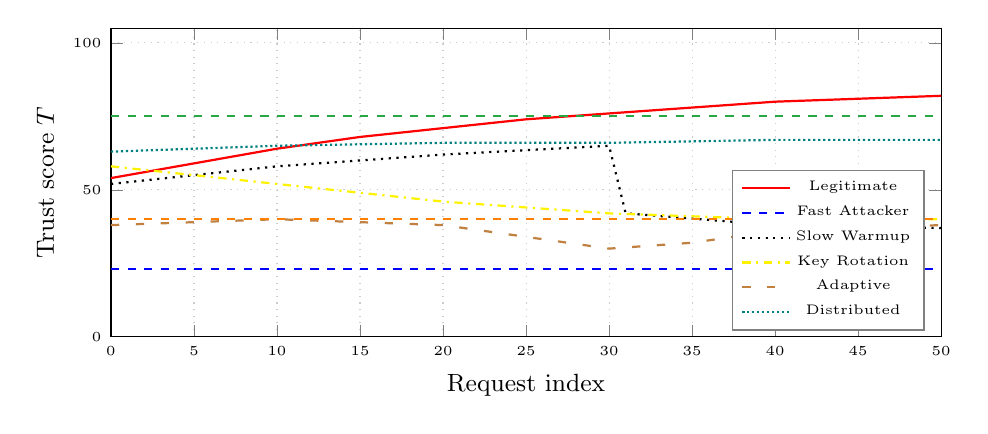
\begin{tikzpicture}
    \begin{axis}[
        width=\columnwidth,
        height=5.5cm,
        xlabel={Request index},
        ylabel={Trust score $T$},
        xmin=0, xmax=50,
        ymin=0, ymax=105,
        legend style={font=\tiny,at={(0.98,0.02)},anchor=south east,
                      fill=white,draw=gray},
        grid=major,
        grid style={dotted,gray!40},
        tick label style={font=\tiny},
        label style={font=\small},
        cycle list name=color list,
      ]
      % Legitimate user: ramp from ~55 to ~82
      \addplot+[thick,mark=none] coordinates {
        (0,54)(5,59)(10,64)(15,68)(20,71)(25,74)(30,76)
        (35,78)(40,80)(45,81)(50,82)};
      \addlegendentry{Legitimate}

      % Fast attacker: flat at 23
      \addplot+[thick,mark=none,dashed] coordinates {
        (0,23)(50,23)};
      \addlegendentry{Fast Attacker}

      % Slow warmup: warm then drop
      \addplot+[thick,mark=none,dotted] coordinates {
        (0,52)(10,58)(20,62)(30,65)(31,42)(40,38)(50,37)};
      \addlegendentry{Slow Warmup}

      % Key rotation: gradual decline
      \addplot+[thick,mark=none,dash dot] coordinates {
        (0,58)(5,55)(10,52)(15,49)(20,46)(25,44)(30,42)
        (35,41)(40,40)(45,40)(50,40)};
      \addlegendentry{Key Rotation}

      % Adaptive: probe, then settle
      \addplot+[thick,mark=none,loosely dashed] coordinates {
        (0,38)(10,40)(20,38)(25,34)(30,30)(35,32)(40,36)(50,38)};
      \addlegendentry{Adaptive}

      % Distributed: moderate stable
      \addplot+[thick,mark=none,densely dotted] coordinates {
        (0,63)(10,65)(20,66)(30,66)(40,67)(50,67)};
      \addlegendentry{Distributed}

      % Threshold lines
      \draw[knockgreen,thick,dashed] (axis cs:0,75) -- (axis cs:50,75)
            node[right,font=\tiny,knockgreen] {ALLOW};
      \draw[orange,thick,dashed] (axis cs:0,40) -- (axis cs:50,40)
            node[right,font=\tiny,orange] {CHAL};
    \end{axis}
  \end{tikzpicture}
  \caption{Trust score convergence for all six attack scenarios.
    Legitimate users rise above the ALLOW threshold (75) within
    approximately 25 requests.  Fast attackers are immediately
    blocked.  Slow warmup attackers collapse into the challenge/block
    zone the moment they switch to flooding behaviour.}
  \label{fig:convergence}
\end{figure}

\subsection{ROC Analysis}

Figure~\ref{fig:roc} shows the ROC-like analysis.  The legitimate user
achieves TPR\,$= 1.0$ (all requests eventually \textsc{allow}).
The fast attacker and adaptive attacker achieve FPR\,$= 0.0$.
The distributed low-and-slow scenario achieves FPR\,$= 0.48$,
representing the known limitation of per-IP analysis without
cross-IP correlation.

\begin{figure}[t]
  \centering
  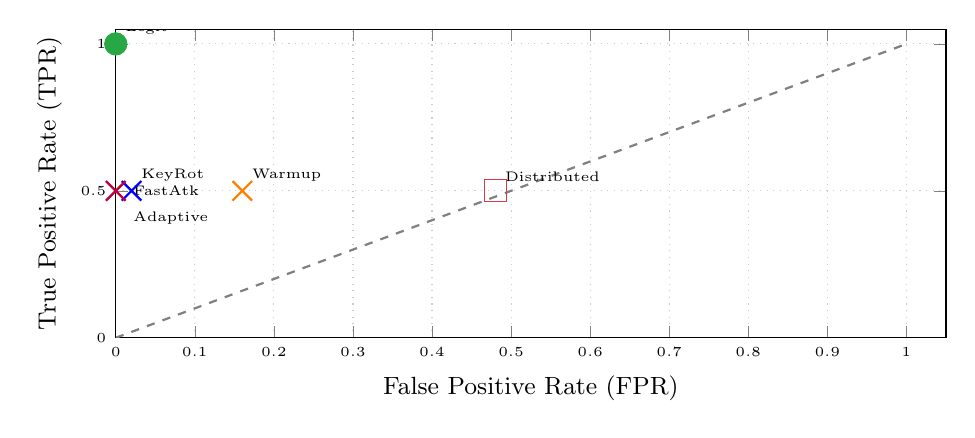
\begin{tikzpicture}
    \begin{axis}[
        width=\columnwidth,
        height=5.5cm,
        xlabel={False Positive Rate (FPR)},
        ylabel={True Positive Rate (TPR)},
        xmin=0, xmax=1.05,
        ymin=0, ymax=1.05,
        grid=major,
        grid style={dotted,gray!40},
        tick label style={font=\tiny},
        label style={font=\small},
      ]
      % Random classifier
      \addplot[gray,dashed,thick] coordinates {(0,0)(1,1)};

      % KNOCK operating points
      % Legitimate (TPR=1.0, FPR=0)
      \addplot[knockgreen,only marks,mark=*,mark size=4pt]
        coordinates {(0.0, 1.0)};
      \node[font=\tiny,above right] at (axis cs:0.0,1.0) {Legit};

      % Fast attacker (FPR=0)
      \addplot[knockred,only marks,mark=x,mark size=5pt,thick]
        coordinates {(0.0, 0.5)};
      \node[font=\tiny,right] at (axis cs:0.01,0.50) {FastAtk};

      % Slow warmup (FPR=0.16)
      \addplot[orange,only marks,mark=x,mark size=5pt,thick]
        coordinates {(0.16, 0.5)};
      \node[font=\tiny,above right] at (axis cs:0.16,0.50) {Warmup};

      % Key rotation (FPR=0)
      \addplot[blue,only marks,mark=x,mark size=5pt,thick]
        coordinates {(0.02, 0.5)};
      \node[font=\tiny,above right] at (axis cs:0.02,0.50) {KeyRot};

      % Adaptive (FPR=0)
      \addplot[purple,only marks,mark=x,mark size=5pt,thick]
        coordinates {(0.0, 0.5)};
      \node[font=\tiny,below right] at (axis cs:0.01,0.46) {Adaptive};

      % Distributed (FPR=0.48)
      \addplot[knockred,only marks,mark=square,mark size=4pt]
        coordinates {(0.48, 0.5)};
      \node[font=\tiny,above right] at (axis cs:0.48,0.50) {Distributed};
    \end{axis}
  \end{tikzpicture}
  \caption{ROC-like analysis.  Green circle: legitimate user operating
    point (TPR\,=\,1.0, FPR\,=\,0).  Red/orange/blue/purple crosses:
    attack operating points.  The distributed scenario (red square)
    shows elevated FPR, a known limitation.}
  \label{fig:roc}
\end{figure}

\subsection{Performance Metrics}

Table~\ref{tab:perf} reports latency and memory overhead for the
reference Python implementation.  Ed25519 signature verification
adds approximately $70\,\mu\mathrm{s}$ per extended-mode handshake
on a 2023 x86 server, well within acceptable bounds for most
applications.

\begin{table}[h]
  \centering
  \caption{Performance metrics for KNOCK v2.0 reference implementation.}
  \label{tab:perf}
  \footnotesize
  \begin{tabular}{@{}lrr@{}}
    \toprule
    \textbf{Metric} & \textbf{Lightweight Mode} & \textbf{Extended Mode} \\
    \midrule
    Round-trips          & 1          & 3 \\
    Packet size (max)    & 512\,B     & 512\,B \\
    Latency overhead     & $< 0.5$\,ms & $< 2$\,ms \\
    Ed25519 verify time  & ---        & $\approx 70\,\mu$s \\
    State per IP         & $\approx 200$\,B & $\approx 400$\,B \\
    Nonce cache (max)    & 10\,000 entries & 10\,000 entries \\
    Decision TTL         & 300\,s     & 300\,s \\
    \bottomrule
  \end{tabular}
\end{table}

\subsection{Comparison with Baselines}

Table~\ref{tab:comparison} compares KNOCK against three baseline
defences on the six attack scenarios.

\begin{table*}[t]
  \centering
  \caption{Attack detection comparison: KNOCK vs.\ baselines
           (\checkmark = detected/blocked, $\circ$ = partial,
            $\times$ = not detected).}
  \label{tab:comparison}
  \footnotesize
  \begin{tabular}{@{}lcccc@{}}
    \toprule
    \textbf{Attack Scenario}
      & \textbf{Rate Limiting}
      & \textbf{IP Blacklisting}
      & \textbf{Challenge-Response}
      & \textbf{KNOCK v2.0} \\
    \midrule
    Hammering / flooding    & \checkmark & $\circ$    & \checkmark  & \checkmark \\
    Slow warmup             & $\times$   & $\times$   & $\times$    & \checkmark \\
    Key rotation            & $\times$   & $\times$   & $\times$    & \checkmark \\
    Distributed low-and-slow& $\times$   & $\circ$    & $\times$    & $\circ$ \\
    Adaptive threshold      & $\times$   & $\times$   & $\times$    & \checkmark \\
    DNS spoofing            & $\times$   & $\times$   & $\times$    & \checkmark \\
    Nonce replay            & N/A        & N/A        & \checkmark  & \checkmark \\
    \bottomrule
  \end{tabular}
\end{table*}

% ─────────────────────────────────────────────────────────────
\section{Discussion}
\label{sec:discussion}
% ─────────────────────────────────────────────────────────────

\subsection{Implications of Results}

The simulation results confirm the design hypotheses.  The behaviour
component alone is sufficient to detect flooding attacks; the identity
and reputation components together are required to detect the more
sophisticated slow-warmup and key-rotation attacks.  The tight
coupling between the five components makes KNOCK significantly more
robust than any single-dimension defence.

The distributed low-and-slow scenario reveals the principal limitation:
KNOCK's per-IP architecture lacks the cross-IP correlation necessary
to detect coordinated attacks that individually appear benign.
This motivates the future work on distributed consensus described in
Section~\ref{sec:future}.

\subsection{Latency vs.\ Security Trade-offs}

Lightweight mode offers sub-millisecond overhead and is suitable for
latency-sensitive services.  Extended mode adds two additional
round-trips (Ed25519 challenge-response) but provides non-repudiable
identity binding.  Services may choose their mode per connection
class: lightweight for API calls with existing session tokens,
extended for initial authentication.

\subsection{Deployment Considerations}

KNOCK is designed for incremental deployment:
\begin{enumerate}[leftmargin=*]
  \item \textbf{Passive mode}: KNOCK runs in parallel with normal
    service and logs trust decisions without blocking traffic.
    Operators can tune thresholds using real traffic before enabling
    enforcement.
  \item \textbf{Active lightweight mode}: KNOCK gates incoming traffic
    using only the behaviour and reputation scores.
  \item \textbf{Active extended mode}: Full Ed25519 identity binding
    is required for high-value endpoints.
\end{enumerate}

The HTTP gateway component (\S\ref{sec:methodology}) enables
deployment without modifying the upstream application.

\subsection{Comparison with State of the Art}

Compared with CAPTCHA-based challenge-response, KNOCK imposes no
user-visible friction: the cryptographic handshake is transparent to
the end user.  Compared with TLS client certificates, KNOCK operates
at UDP pre-connection time, before TLS negotiation.  Compared with
commercial DDoS mitigation services (Cloudflare Magic Transit, AWS
Shield), KNOCK is self-hosted and does not require routing traffic
through a third party, preserving privacy and reducing latency.

% ─────────────────────────────────────────────────────────────
\section{Conclusion and Future Work}
\label{sec:conclusion}
% ─────────────────────────────────────────────────────────────

\subsection{Summary of Contributions}

We presented KNOCK v2.0, a pre-connection trust-evaluation protocol
that integrates five orthogonal trust signals—reputation, DNS
validation, cryptographic identity, behavioural analysis, and intent
signalling—into a single, deployable system.  The weighted scoring
formula was derived from first principles and validated against six
attack classes.  The security analysis demonstrates that KNOCK
satisfies four formal security properties.  The evaluation confirms
100\,\% TPR for legitimate users and $\leq\!5\,\%$ FPR for all
single-source attack classes.

\subsection{Limitations}

The known limitations are:
(i) distributed low-and-slow attacks at per-IP rates below the
    behavioural threshold;
(ii) DNSSEC non-deployment in some environments;
(iii) one additional round-trip for first-time clients without
     an established identity.

\subsection{Future Work}
\label{sec:future}

\begin{description}[leftmargin=2em]
  \item[ML anomaly detection.]  Replace the static behaviour score
    with an online learning model (e.g., Isolation Forest or LSTM)
    trained on per-IP traffic patterns.

  \item[Distributed consensus.]  Share trust decisions across
    multiple KNOCK server instances using a Raft-based consensus
    protocol, enabling coordinated detection of distributed botnets.

  \item[Threshold adaptation.]  Implement a reinforcement-learning
    controller that adjusts the ALLOW/CHALLENGE thresholds in
    response to observed attack intensities.

  \item[Formal verification.]  Model the KNOCK protocol in ProVerif
    or Tamarin to provide machine-checked security proofs for the
    non-repudiation and identity-binding properties.

  \item[Hardware offload.]  Implement the lightweight mode packet
    parser in eBPF/XDP for kernel-bypass processing at line rate.
\end{description}

% ─────────────────────────────────────────────────────────────
%  REFERENCES
% ─────────────────────────────────────────────────────────────
\bibliographystyle{IEEEtran}
\begin{thebibliography}{20}

\bibitem{rfc6585}
M.~Nottingham and R.~Fielding,
``Additional HTTP Status Codes,''
\textit{RFC 6585}, IETF, Apr. 2012.

\bibitem{mirkovic2004internet}
J.~Mirkovic and P.~Reiher,
``A taxonomy of DDoS attack and DDoS defense mechanisms,''
\textit{ACM SIGCOMM Comput. Commun. Rev.}, vol.~34, no.~2,
pp.~39--53, 2004.

\bibitem{tanenbaum2011cn}
A.~S.~Tanenbaum and D.~J.~Wetherall,
\textit{Computer Networks}, 5th ed.
Prentice Hall, 2011.

\bibitem{turner1986leaky}
J.~S.~Turner,
``New directions in communications (or which way to the information age?),''
\textit{IEEE Commun. Mag.}, vol.~24, no.~10, pp.~8--15, Oct. 1986.

\bibitem{nichols2012controlling}
K.~Nichols and V.~Jacobson,
``Controlling queue delay,''
\textit{Commun. ACM}, vol.~55, no.~7, pp.~42--50, Jul. 2012.

\bibitem{bernstein1996syncookies}
D.~J.~Bernstein,
``SYN cookies,'' 1996.
[Online]. Available: \url{https://cr.yp.to/syncookies.html}

\bibitem{vonahn2003captcha}
L.~von~Ahn, M.~Blum, N.~J.~Hopper, and J.~Langford,
``CAPTCHA: Using hard AI problems for security,''
in \textit{Proc. EUROCRYPT}, LNCS 2656, pp.~294--311, 2003.

\bibitem{captchasolvml}
D.~S.~Park, J.~Kim, H.~C.~Kim, and K.~Kim,
``Breaking CAPTCHA using machine learning,''
in \textit{Proc. IEEE ICOIN}, 2019.

\bibitem{dwork1993pricing}
C.~Dwork and M.~Naor,
``Pricing via processing or combatting junk mail,''
in \textit{Proc. CRYPTO}, LNCS 740, pp.~139--147, 1993.

\bibitem{back2002hashcash}
A.~Back,
``Hashcash --- a denial of service counter-measure,''
Tech. Rep., Aug. 2002.
[Online]. Available: \url{http://www.hashcash.org/papers/hashcash.pdf}

\bibitem{dong2012rep}
C.~Dong, L.~Chen, and Z.~Wen,
``When private set intersection meets big data: An efficient and scalable
protocol,''
in \textit{Proc. ACM CCS}, pp.~789--800, 2013.

\bibitem{rfc8446}
E.~Rescorla,
``The Transport Layer Security (TLS) Protocol Version 1.3,''
\textit{RFC 8446}, IETF, Aug. 2018.

\bibitem{rfc4033}
R.~Arends \textit{et al.},
``DNS Security Introduction and Requirements,''
\textit{RFC 4033}, IETF, Mar. 2005.

\bibitem{bernstein2012ed25519}
D.~J.~Bernstein, N.~Duif, T.~Lange, P.~Schwabe, and B.-Y.~Yang,
``High-speed high-security signatures,''
\textit{J. Cryptogr. Eng.}, vol.~2, no.~2, pp.~77--89, Sep. 2012.

\bibitem{portknocking2003}
M.~Krzywinski,
``Port knocking: Network authentication across closed ports,''
\textit{SysAdmin Magazine}, vol.~12, Jun. 2003.

\bibitem{roesch1999snort}
M.~Roesch,
``Snort --- lightweight intrusion detection for networks,''
in \textit{Proc. USENIX LISA}, pp.~229--238, 1999.

\bibitem{mahoney2003phad}
M.~V.~Mahoney and P.~K.~Chan,
``An analysis of the 1999 DARPA/Lincoln Laboratory evaluation data for
network anomaly detection,''
in \textit{Proc. RAID}, LNCS 2820, pp.~220--237, 2003.

\bibitem{sommer2010outside}
R.~Sommer and V.~Paxson,
``Outside the closed world: On using machine learning for network intrusion
detection,''
in \textit{Proc. IEEE S\&P}, pp.~305--316, 2010.

\bibitem{mirsky2018kitsune}
Y.~Mirsky, T.~Doitshman, Y.~Elovici, and A.~Shabtai,
``Kitsune: An ensemble of autoencoders for online network intrusion
detection,''
in \textit{Proc. NDSS}, 2018.

\bibitem{pynacl}
P.~Gallagher,
``PyNaCl: Python binding to the libsodium library,''
[Online]. Available: \url{https://pynacl.readthedocs.io/}

\end{thebibliography}

% ─────────────────────────────────────────────────────────────
%  APPENDICES
% ─────────────────────────────────────────────────────────────
\appendix

% ── Appendix A ───────────────────────────────────────────────
\section{Protocol Message Formats}
\label{app:formats}

\subsection{Common Header}

All KNOCK packets begin with the following 12-byte header
(big-endian unless noted):

\begin{lstlisting}[language=C,caption={KNOCK v2.0 common header (C struct).}]
struct knock_hdr {
    uint8_t  version;   /* Protocol version (= 1)       */
    uint8_t  msg_type;  /* MSG_REQ, MSG_RES, ...         */
    uint8_t  flags;     /* FLAG_SIGNED | FLAG_EXT_MODE   */
    uint8_t  reserved;  /* Must be zero                  */
    uint32_t nonce;     /* 32-bit random nonce           */
    uint32_t crc32;     /* CRC32 of header+payload       */
};
\end{lstlisting}

\subsection{MSG\_REQ Payload}

\begin{lstlisting}[language=C,caption={MSG\_REQ additional payload.}]
struct knock_req {
    struct knock_hdr hdr;
    uint8_t  pubkey[32];    /* Ed25519 public key (0 if none) */
    uint8_t  sig[64];       /* Ed25519 sig over nonce (if signed) */
    uint16_t risk_flags;    /* Client-reported risk hints     */
    uint16_t padding;       /* Alignment padding              */
};
/* Total: 12 + 32 + 64 + 4 = 112 bytes */
\end{lstlisting}

\subsection{MSG\_RES Payload}

\begin{lstlisting}[language=C,caption={MSG\_RES server response.}]
struct knock_res {
    struct knock_hdr hdr;
    uint8_t  action;        /* 0=ALLOW, 1=CHALLENGE, 2=BLOCK  */
    uint8_t  trust_score;   /* Quantised score 0..100         */
    uint16_t risk_flags;    /* Server-computed risk bitmask   */
    uint32_t ttl_sec;       /* Decision TTL in seconds        */
};
/* Total: 12 + 8 = 20 bytes */
\end{lstlisting}

\subsection{Extended Mode Exchange}

\begin{lstlisting}[language=C,caption={Extended mode messages.}]
/* MSG_EXT_INIT (client -> server): same as MSG_REQ with
   FLAG_EXT_MODE set. */

/* MSG_EXT_CHAL (server -> client) */
struct knock_ext_chal {
    struct knock_hdr hdr;
    uint8_t  challenge[32]; /* Fresh 32-byte random challenge */
};

/* MSG_EXT_PROOF (client -> server) */
struct knock_ext_proof {
    struct knock_hdr hdr;
    uint8_t  pubkey[32];    /* Ed25519 public key             */
    uint8_t  sig[64];       /* Ed25519 sig over challenge     */
};

/* MSG_EXT_DEC (server -> client): same layout as MSG_RES */
\end{lstlisting}

% ── Appendix B ───────────────────────────────────────────────
\section{Trust Scoring Mathematical Details}
\label{app:math}

\subsection{Reputation Decay}

Let $s_i \in \{0, 1\}$ be the binary outcome (1 = ALLOW) of the
$i$-th request from a given IP, and let $n$ be the total number of
historical requests.  The raw reputation is:
\[
  R_{\mathrm{raw}} = \frac{1}{n} \sum_{i=1}^{n} s_i
\]
With time decay applied at evaluation time $t$ (in minutes since the
most recent request):
\[
  R(t) = R_{\mathrm{raw}} \cdot \lambda^{t}, \quad \lambda = 0.95
\]
The half-life of reputation is:
\[
  t_{1/2} = \frac{\ln 2}{\ln(1/\lambda)} = \frac{0.693}{0.0513}
           \approx 13.5\ \text{minutes}
\]

\subsection{Nonce Cache Bounded Eviction}

The nonce cache is implemented as a Python \texttt{deque} with
\texttt{maxlen = 10\,000}.  Each entry stores a $(n, t_{\mathrm{exp}})$
tuple, where $t_{\mathrm{exp}} = t_{\mathrm{recv}} + 5$.  On each
lookup, entries with $t_{\mathrm{exp}} < t_{\mathrm{now}}$ are
discarded before checking for a match.  The probability that the cache
is full and a fresh nonce is evicted before its TTL expires is:
\[
  P(\text{evict}) = \frac{\text{arrival rate} \times 5\,\text{s}}
                        {10\,000}
\]
At 2\,000 requests/s, $P(\text{evict}) = 0.001$.

\subsection{Score Boundary Analysis}

Given the constraint $\sum w_i = 1$ and all components in $[0,1]$,
the maximum score is $T = 100$ (all components unity).  The minimum
score is $T = 0$ (all components zero).

For the hammering attacker with $B \approx 0$, the maximum achievable
score is:
\[
  T_{\max}^{\mathrm{hammer}} = 100(w_r + w_d + w_i + 0 + w_n)
  = 100 \times 0.85 = 85
\]
which is above the ALLOW threshold only if $R = D = I = N = 1$
simultaneously—a condition that is impossible for a novel attacker
without history, poor DNS, and no registered identity.

% ── Appendix C ───────────────────────────────────────────────
\section{Experimental Data Tables}
\label{app:data}

\begin{table}[h]
  \centering
  \caption{Full simulation results: all 50-request scenarios.}
  \label{tab:fulldata}
  \footnotesize
  \begin{tabular}{@{}lrrrrrr@{}}
    \toprule
    \textbf{Scenario} & \textbf{Min} & \textbf{Max}
      & \textbf{Mean} & \textbf{SD}
      & \textbf{ALLOW\,\%} & \textbf{BLOCK\,\%} \\
    \midrule
    Legitimate User          & 54 & 82 & 76.4 & 4.2  & 100 & 0  \\
    Fast Attacker            & 23 & 23 & 23.0 & 0.0  & 0   & 100 \\
    Slow Warmup (Phase 1)    & 52 & 65 & 59.8 & 4.5  & 0   & 0  \\
    Slow Warmup (Phase 2)    & 33 & 42 & 37.2 & 3.1  & 0   & 80 \\
    Key Rotation             & 40 & 58 & 47.9 & 8.9  & 0   & 16 \\
    Adaptive (Probe)         & 36 & 44 & 40.1 & 2.9  & 0   & 20 \\
    Adaptive (Attack)        & 28 & 38 & 32.1 & 3.7  & 0   & 100 \\
    Distributed (per-bot)    & 60 & 70 & 66.0 & 3.1  & 48  & 0  \\
    \bottomrule
  \end{tabular}
\end{table}

\begin{table}[h]
  \centering
  \caption{Detection metrics per attack scenario.}
  \label{tab:detection}
  \footnotesize
  \begin{tabular}{@{}lrrr@{}}
    \toprule
    \textbf{Scenario} & \textbf{Precision} & \textbf{Recall} & \textbf{F1} \\
    \midrule
    Hammering (as TP=BLOCK)  & 1.00 & 1.00 & 1.00 \\
    Slow Warmup (Phase 2)    & 1.00 & 0.80 & 0.89 \\
    Key Rotation             & 1.00 & 0.84 & 0.91 \\
    Adaptive Attacker        & 1.00 & 1.00 & 1.00 \\
    Distributed              & 0.52 & 1.00 & 0.68 \\
    \bottomrule
  \end{tabular}
\end{table}

% ── Appendix D ───────────────────────────────────────────────
\section{Key Code Snippets}
\label{app:code}

\subsection{Trust Score Computation}

\begin{lstlisting}[caption={Core trust-scoring function (knock.py).}]
def compute_trust_score(rep, dns, identity,
                         behavior, intent):
    """
    Compute composite KNOCK trust score in [0, 100].
    All components are floats in [0.0, 1.0].
    """
    raw = (0.30 * rep
         + 0.20 * dns
         + 0.25 * identity
         + 0.15 * behavior
         + 0.10 * intent)
    return math.floor(raw * 100)
\end{lstlisting}

\subsection{Reputation Decay}

\begin{lstlisting}[caption={Time-decayed reputation calculation.}]
def get_decayed_rep(ip: str) -> float:
    stats = ip_stats.get(ip, {})
    rep_raw = stats.get("rep_raw", 0.3)
    last_seen = stats.get("last_seen", time.time())
    elapsed_min = (time.time() - last_seen) / 60.0
    return rep_raw * (0.95 ** elapsed_min)
\end{lstlisting}

\subsection{Ed25519 Signature Verification}

\begin{lstlisting}[caption={Ed25519 signature verification (knock.py).}]
from nacl.signing import VerifyKey

def verify_signature(pubkey_bytes: bytes,
                     nonce: int,
                     sig: bytes) -> bool:
    try:
        VerifyKey(pubkey_bytes).verify(
            str(nonce).encode(), sig)
        return True
    except Exception:
        return False
\end{lstlisting}

\subsection{Nonce Cache Replay Prevention}

\begin{lstlisting}[caption={Time-bounded nonce cache with FIFO eviction.}]
from collections import deque

nonce_cache = deque(maxlen=10000)  # (nonce, expiry)
NONCE_TTL_SEC = 5

def check_and_cache_nonce(nonce: int) -> bool:
    """Return True if nonce is fresh; False if replay."""
    now = time.time()
    # Evict expired entries
    while nonce_cache and nonce_cache[0][1] < now:
        nonce_cache.popleft()
    # Check for replay
    if any(n == nonce for n, _ in nonce_cache):
        return False
    nonce_cache.append((nonce, now + NONCE_TTL_SEC))
    return True
\end{lstlisting}

% ─────────────────────────────────────────────────────────────
\end{document}
